\documentclass[fontset=windows,12pt]{article}

\usepackage[UTF8]{ctex}
\usepackage[a4paper]{geometry}
\usepackage{amsmath}
\usepackage{fancyhdr}
\usepackage{amsthm}
\usepackage{amssymb}
\usepackage{xcolor}
\usepackage{listings}
\usepackage{graphicx}
\usepackage{circuitikz}
\ctikzset{logic ports=ieee}     %所有逻辑门使用IEEE标准
\usetikzlibrary{calc}           %使用TikZ中的计算功能
\setlength{\headheight}{14.49998pt}

\newtheorem{question}{\hskip 1.7mm \bf}
\renewenvironment{proof}{{\noindent\hskip 2em \bf ֤证明 \quad}}{\hfill$\qed$\par}
\newenvironment{solution}{{\noindent\hskip 2.4em \bf 解 \quad}}

\geometry{left=2.0cm,right=2.0cm,top=2.5cm,bottom=2.5cm}
\begin{document}

\definecolor{CPPLight}  {HTML} {686868}
\definecolor{CPPSteel}  {HTML} {888888}
\definecolor{CPPDark}   {HTML} {262626}
\definecolor{CPPBlue}   {HTML} {4172A3}
\definecolor{CPPGreen}  {HTML} {487818}
\definecolor{CPPBrown}  {HTML} {A07040}
\definecolor{CPPRed}    {HTML} {AD4D3A}
\definecolor{CPPViolet} {HTML} {7040A0}
\definecolor{CPPGray}  {HTML} {B8B8B8}
\lstset{
    columns=fixed,       
    numbers=left,                                        % 在左侧显示行号
    frame=none,                                          % 不显示背景边框
    backgroundcolor=\color[RGB]{245,245,244},            % 设定背景颜色
    keywordstyle=\color[RGB]{40,40,255},                 % 设定关键字颜色
    numberstyle=\footnotesize\color{darkgray},           % 设定行号格式
    commentstyle=\it\color[RGB]{0,96,96},                % 设置代码注释的格式
    stringstyle=\rmfamily\slshape\color[RGB]{128,0,0},   % 设置字符串格式
    showstringspaces=false,                              % 不显示字符串中的空格
    language=c++,                                        % 设置语言
    morekeywords={alignas,continute,friend,register,true,alignof,decltype,goto,
    reinterpret_cast,try,asm,defult,if,return,typedef,auto,delete,inline,short,
    typeid,bool,do,int,signed,typename,break,double,long,sizeof,union,case,
    dynamic_cast,mutable,static,unsigned,catch,else,namespace,static_assert,using,
    char,enum,new,static_cast,virtual,char16_t,char32_t,explict,noexcept,struct,
    void,export,nullptr,switch,volatile,class,extern,operator,template,wchar_t,
    const,false,private,this,while,constexpr,float,protected,thread_local,
    const_cast,for,public,throw,std},
    emph={map,set,multimap,multiset,unordered_map,unordered_set,
    unordered_multiset,unordered_multimap,vector,string,list,deque,
    array,stack,forwared_list,iostream,memory,shared_ptr,unique_ptr,
    random,bitset,ostream,istream,cout,cin,endl,move,default_random_engine,
    uniform_int_distribution,iterator,algorithm,functional,bing,numeric,},
    emphstyle=\color{CPPViolet}, 
}
\newenvironment{correction}{\par\noindent{\color{blue}{\bf{更正\\}}}\quad\color{blue}}{\par}
\pagestyle{fancy}
\lhead{中国科学院大学}
\chead{\bf{2024-25秋数字电路课程}}
\rhead{\emph{2023K8009929044 薛翼舟}}


\begin{center}
\huge{\bf{实验报告1}}
\end{center}

\section{实验目的}
    \subsection{熟悉vivado环境}
    数是vivado设计流程, 掌握利用vivado创建设计的方法, 掌握编写testbench的方法(利用testbench来测试设计), 掌握行为仿真法
    \subsection{掌握基本的vivado设计编写}
    以四位全加加器以及3-8译码器为例, 熟悉并掌握基本的设计编写思路

\section{实验环境}
    AMD Vivado2022.2

\section{原理说明}
    \subsection{四位全加器(利用门电路实现一位加法器)}
    考虑全加器, 输入为A,B,Cin,输出为本位输出S和进位输出Cout
    \begin{align*}
        S=A\oplus B\oplus Cin
    \end{align*}
    经过测试, 在verilog语言中无法进行三个异或, 因此需要声明一个wire w1在存前两个异或, 以实现三个异或
    \begin{align*}
        Cout=(A\oplus B)\cdot Cin+A\cdot B\cdot Cin
    \end{align*}
    门电路图如下\\ 
    \begin{center}
        \begin{circuitikz}[scale=0.7, transform shape]
            \draw (10,5.5) node[xor port, anchor=out] (xor1) {};
            \draw (15,4.7) node[xor port, anchor=out] (xor2) {};
            \draw (15.5,3) node[and port, anchor=out] (and1) {};
            \draw (10.5,2) node[and port, anchor=out] (and2) {};
            \draw (18,2.5) node[or port, anchor=out] (or) {};
            \draw(xor1.out) |- (xor2.in 1);
            \draw(and1.out) |- (or.in 1);
            \draw(and2.out) |- (or.in 2);


            \draw let \p1=(xor1.in 1) in (\x1,\y1) -- (6,\y1) node(A)[left,scale={1/0.7}] {$A$};
            \draw let \p1=(xor1.in 2) in (\x1,\y1) -- (6,\y1) node(B)[left,scale={1/0.7}] {$B$};
            \draw let \p1=(xor2.in 2) in (\x1,\y1) -- (6,\y1) node(Cin)[left,scale={1/0.7}] {$Cin$};
            \draw let \p1=(xor2.out) in (\x1,\y1) -- (18.5,\y1) node(A)[right,scale={1/0.7}] {$S$};
            \draw let \p1=(or.out) in (\x1,\y1) -- (18.5,\y1) node(A)[right,scale={1/0.7}] {$Cout$};

            \draw let \p1=(xor1.in 1),\p2=(A) in (\x1,\y1) to[short,-*] (6.5,\y1) node (a) {};
            \draw let \p1=(xor1.in 2),\p2=(B) in (\x1,\y1) to[short,-*] (7,\y1) node (b) {};
            \draw let \p1=(xor2.in 2),\p2=(Cin) in (\x1,\y1) to[short,-*] (10.5,\y1) node (c) {};
            \draw let \p1=(10,5), in (\x1,\y1) to[short,-*] (11,5) node (d) {};


            \draw(a) |- (and2.in 1);
            \draw(b) |- (and2.in 2);
            \draw(c) |- (and1.in 2);
            \draw(d) |- (and1.in 1);
        \end{circuitikz}
    \end{center}

    \subsection{3-8译码器}
        输入的是一个三位的二进制数, 而这个电路是高电平有效的, 因此在state=1时才执行译码, 否则全部都是未驱动. 直接采取一一对应的电路, 电路图如下(采取0输出有效)\\
        \begin{figure}[ht]
            \centering
            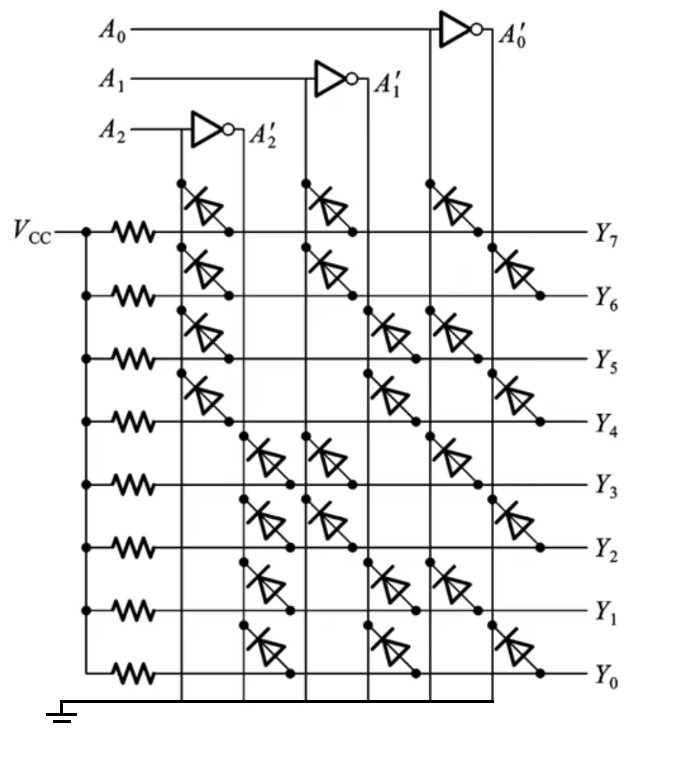
\includegraphics[width=0.8\textwidth]{3to8decoder.jpg}
            \label{3to8decoder}
        \end{figure}\par
        在这里提出一种想法, 每次读取输入的最低位, 然后根据0和1的不同来选取可能的结果, 之后再将输入右移1, 重复此过程, 例如输入是101, 最低位是1, 则有可能是1,3,5,7, 
        右移变为010, 最低为是0, 则有可能是1,5, 以此类推(这样可能比较符合程序的逻辑, 但在电路中的实现貌似更麻烦)
        \bigskip\bigskip\bigskip\bigskip
\section{接口定义}
    \subsection{4位全加器}
    {\setmainfont{Courier New Bold}                          % 设置代码字体                   
    \begin{lstlisting}
    输入:
        [3:0]in_0   (四位输入1)
        [3:0]in_1   (四位输入2)
        c_in    (进位输入)
    输出:
        [3:0]out    (四位输出)
        c_out   (进位输出)
    \end{lstlisting}}
    \subsection{3-8译码器}
    {\setmainfont{Courier New Bold}                          % 设置代码字体                   
    \begin{lstlisting}
    输入:
        [2:0]in   (三位输入)
        state   (有效电平)
    输出:
        [7:0]out    (输出)
    \end{lstlisting}}

\section{调试过程及结果}
    \subsection{4位加法器}
        在四位加法器中并未遇到什么困难, 在这里直接给出结果波形图
        \begin{figure}[ht]
            \centering
            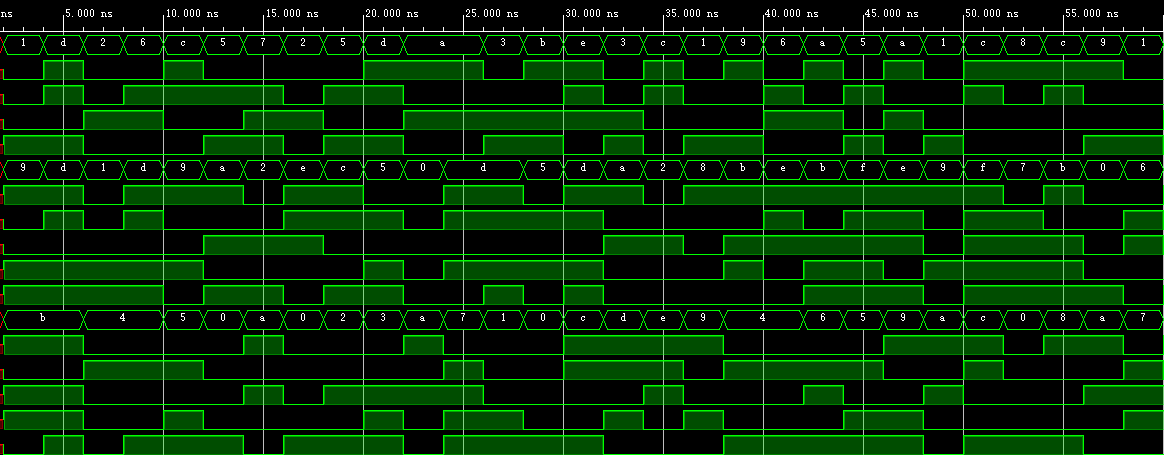
\includegraphics[width=1\textwidth]{add4.jpg}
            \caption{从上到下分别是输入1, 输入2, 进位输入, 输出, 进位输出}
            \label{3to8decoder}
        \end{figure}\par
    \subsection{1位全加器}
        在一位全加器中, 我注意到在verilog语言中不可以利用门进行两个以上的逻辑运算操作, 需要引入线来作为中间变量, 例如存下前两个异或的结果
        再将这个结果与第三个变量做异或得到三个变量异或的结果
        \begin{figure}[ht]
            \centering
            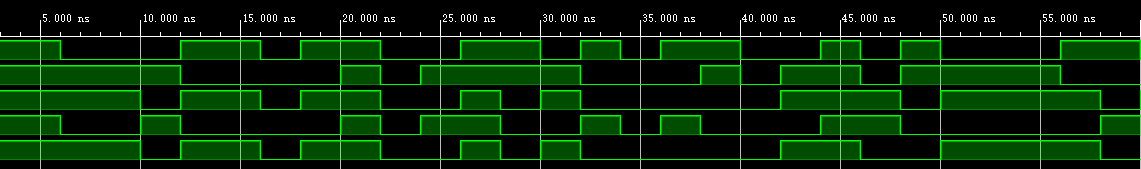
\includegraphics[width=1\textwidth]{add1.jpg}
            \caption{从上到下分别是输入1, 输入2, 进位输入, 本位输出, 进位输出}
            \label{3to8decoder}
        \end{figure}\par
    \subsection{3-8译码器}
        在3=8译码器中, 注意到进行reg时, 不可以在声明端口外进行reg声明, 这样会造成不期望的Z驱动
        \begin{figure}[ht]
            \centering
            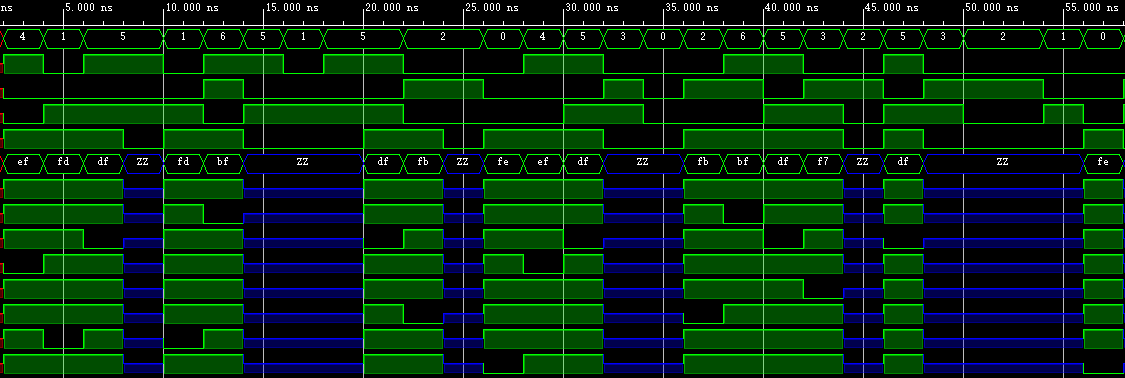
\includegraphics[width=1\textwidth]{decoder.jpg}
            \caption{从上到下分别是3位输入, 有效电平state, 输出}
            \label{3to8decoder}
        \end{figure}\par

\section{实验总结}
    \subsection{Vivado使用方面}
        熟悉了如何创建、编辑、设计工程, 并学会使用了激励文件来测试工程
    \subsection{Verilog语言方面}
        进一步了解了reg的用法、随机数的生成以及always, if, cases的使用

\section{源代码}
    \subsection{四位加法器}
    {\setmainfont{Courier New Bold}                          % 设置代码字体                   
    \begin{lstlisting}
    module add_4(
        input [3:0] in_0,
        input [3:0] in_1,
        input c_in,
        output [3:0] out,
        output cout);
        
        assign{cout, out}=in_0+in_1+c_in;
        
    endmodule
    \end{lstlisting}}
    \subsection{1位全加器}
    {\setmainfont{Courier New Bold}                          % 设置代码字体                   
    \begin{lstlisting}
    module add_1(
        input in_0,
        input in_1,
        input cin,
        output cout,
        output s
        );
        wire x1;
        xor(w1,in_0,in_1);
        xor(s,w1,cin);
        wire y1,y2,y3;
        and(y1,w1,cin);
        and(y2,in_0,in_1);
        and(y3,y2,cin);
        or(cout,y3,y1);
        
    endmodule
    \end{lstlisting}}
    \subsection{3-8译码器}
    {\setmainfont{Courier New Bold}                          % 设置代码字体                   
    \begin{lstlisting}
    module decoder1(
        input [2:0]in,
        input state,
        output reg[7:0]out
        );
    
        always @(state or in)begin
        if(state)begin
            case(in)
                3'b000: out=8'b11111110;
                3'b001: out=8'b11111101;
                3'b010: out=8'b11111011;
                3'b011: out=8'b11110111;
                3'b100: out=8'b11101111;
                3'b101: out=8'b11011111;
                3'b110: out=8'b10111111;
                3'b111: out=8'b01111111;
                default out=8'b11111111;
            endcase
        end
        else 
            out=8'bZZZZZZZZ;
    end
    endmodule
    \end{lstlisting}}
\end{document}      
